\begin{figure*}
    \centering
     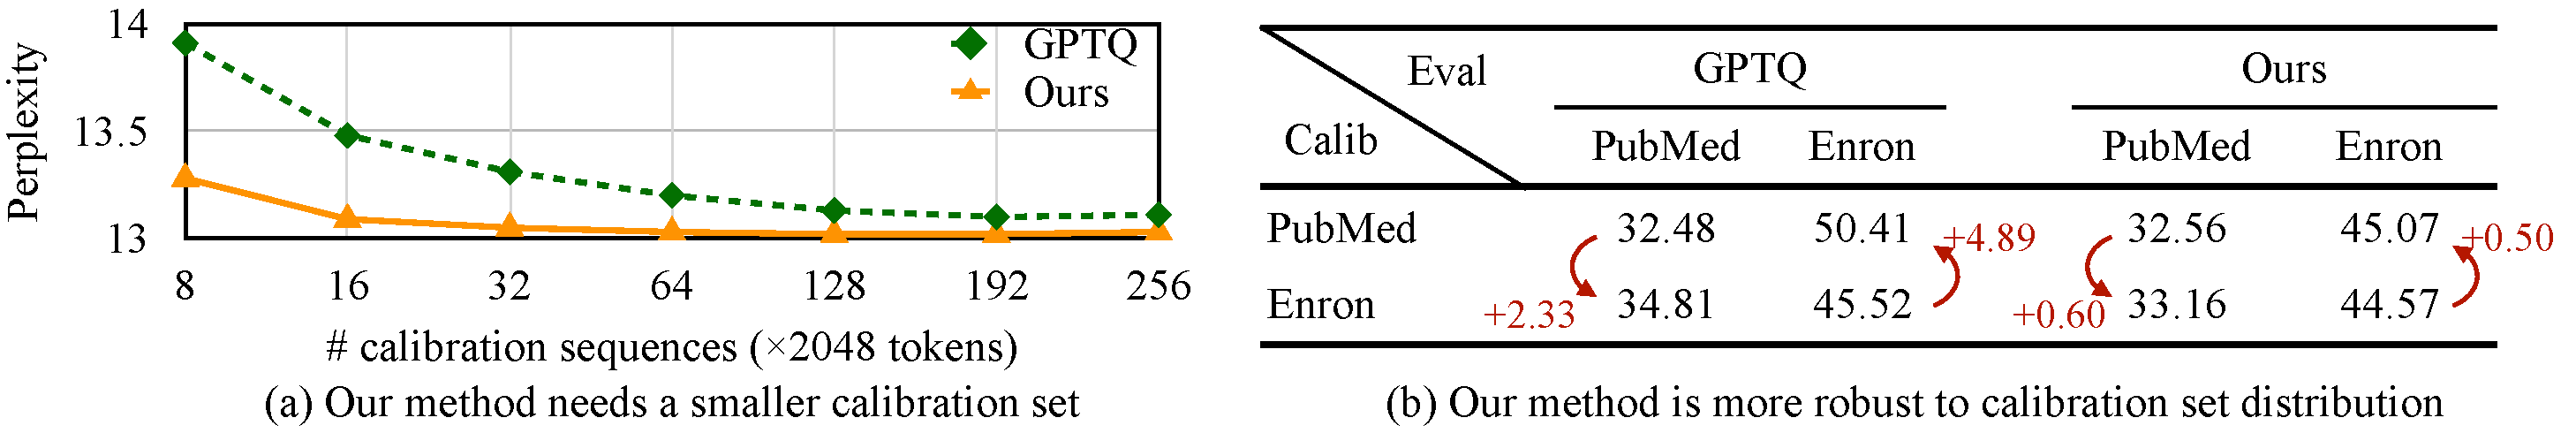
\includegraphics[width=\textwidth]{figures/calib_set_ablation_small.pdf}
    \caption{\textbf{Left:} \methodshort needs a much smaller calibration set to reach a good quantized performance. It can achieve better perplexity using 10$\times$ smaller calibration set compared to GPTQ. \textbf{Right:} Our method is more robust to the calibration set distribution. Overall, using the same calibration and evaluation distribution works the best (PubMed-PubMed, Enron-Enron). But when using a different calibration distribution (PubMed-Enron, Enron-PubMed), \methodshort only increases the perplexity by 0.5-0.6, while GPTQ has 2.3-4.9 worse perplexity. All experiments are done with the OPT-6.7B model under INT3-g128 quantization.}
    \label{fig:calib_set_ablation}
\end{figure*}
